\documentclass[12pt, dvipdfmx]{beamer}

\renewcommand{\kanjifamilydefault}{\gtdefault}
%%%%%%%%%%%  package  %%%%%%%%%%%
\usepackage{bxdpx-beamer}% dvipdfmxなので必要
\usepackage{pxjahyper}% 日本語で'しおり'したい

\usepackage{amssymb,amsmath,ascmac}
\usepackage{derivative}

\usepackage{multirow}
\usepackage{bm}

\graphicspath{{../fig/}}

\usepackage{animate}
\usepackage{tikz}
\usepackage{xparse}

%目次スライド
\AtBeginSection[]{
  \frame{\tableofcontents[currentsection]}
}
%アペンディックスのページ番号除去
\newcommand{\backupbegin}{
\newcounter{framenumberappendix}
\setcounter{framenumberappendix}{\value{framenumber}}
}
\newcommand{\backupend}{
\addtocounter{framenumberappendix}{-\value{framenumber}}
\addtocounter{framenumber}{\value{framenumberappendix}} 
}

%%%%%%%%%%%  theme  %%%%%%%%%%%
\usetheme{Copenhagen}
% \usetheme{Metropolis}
% \usetheme{CambridgeUS}
% \usetheme{Berlin}

%%%%%%%%%%%  inner theme  %%%%%%%%%%%
% \useinnertheme{default}

% %%%%%%%%%%%  outer theme  %%%%%%%%%%%
\useoutertheme{default}
% \useoutertheme{infolines}

%%%%%%%%%%%  color theme  %%%%%%%%%%%
%\usecolortheme{structure}

%%%%%%%%%%%  font theme  %%%%%%%%%%%
\usefonttheme{professionalfonts}
%\usefonttheme{default}

%%%%%%%%%%%  degree of transparency  %%%%%%%%%%%
%\setbeamercovered{transparent=30}

% \setbeamertemplate{items}[default]

%%%%%%%%%%%  numbering  %%%%%%%%%%%
% \setbeamertemplate{numbered}
\setbeamertemplate{navigation symbols}{}
\setbeamertemplate{footline}[frame number]


\title{粘着技術とタッキファイヤーの基礎\\と応用展開}
\subtitle{ ~ 第三章 粘着特性の理解に必要な物理について ~}
\author[東亞合成 佐々木]{佐々木 裕\thanks{hiroshi\_sasaki@mail.toagosei.co.jp}}
\institute[東亞合成]{東亞合成株式会社}
\date{}

\begin{document}

%%%%%
% 1 P
%%%%%
\maketitle

\begin{frame} 
    \tableofcontents[]
\end{frame} 

\section{表面張力と濡れ、そして、相溶性}

\subsection{表面張力と濡れ}
\begin{frame}
	\frametitle{表面張力の古典的な理解}
	\begin{block}{自然現象の観察から}
		\begin{itemize}
			\item 葉の上の水滴の形が丸くなること
			\item コップいっぱいの水がフチを越えて盛り上がること
			\item 一円玉が水に浮かぶこと
		\end{itemize}
		\begin{columns}[c, onlytextwidth]
			\column{.33\linewidth}
			\centering
			\includegraphics[width=.6\textwidth]{waterdrop.png}
			\column{.33\linewidth}
			\centering
			\includegraphics[width=.6\textwidth]{hyoumen_cup.jpg}
			\column{.33\linewidth}
			\centering
			\includegraphics[width=.41\textwidth]{hyoumen_1.png}
		\end{columns}
	\end{block}

	\begin{exampleblock}{上記の現象から、力として理解}
		\begin{itemize}
			\item 液体の表面に張り詰めた力をイメージ
			\item 表面を小さくしようとする力とも考えられた
			\item 「表面の1cmの長さを横切る力 (mN/m)」と定義
		\end{itemize}
	\end{exampleblock}
\end{frame}

\begin{frame}
	\frametitle{Young 式のイメージ}
	\begin{block}{Young 式は、力の釣り合いを考えたもの}
		\begin{columns}[c, onlytextwidth]
			\column{.48\linewidth}
			\begin{align*}
				\gamma_{SV} = \gamma_{LV} \cos \theta + \gamma_{SL}
			\end{align*}
			\column{.48\linewidth}
			\begin{itemize}
				\item $\gamma_{SV}$ は固体⇔空気
				\item $\gamma_{LV}$ は液体⇔空気
				\item $\gamma_{SL}$ は液体⇔固体
			\end{itemize}
		\end{columns}
		
		\vspace{2mm}
		\begin{itemize}
			% \item $\gamma_{SV}$ は固体表面と空気との間での力
			% \item $\gamma_{LV}$ は液体と空気との間の力
			% \item $\gamma_{SL}$ は液体と固体との間の力
			\item 液滴を縮める力($\gamma_{LV} \cos \theta + \gamma_{SL}$)と広げる力($\gamma_{SV}$)の釣り合い
		\end{itemize}

		\centering
			\includegraphics[width=.45\textwidth]{young.png}
	\end{block}
\end{frame}

\begin{frame}
	\frametitle{濡れのイメージ}
	
		\begin{block}{接触角 $\theta$ で濡れを理解}
			\begin{columns}[c, onlytextwidth]
				\column{.6\linewidth}
					\begin{itemize}
						\item $\theta = 90^{o}$: $\gamma_{LV}$ の寄与はない。
						\item $\theta < 90^{o}$: 固体は気体と接するよりも液体の方が好き。
						\item $\theta > 90^{o}$: 固体は気体と接するほうが居心地がいい。
					\end{itemize}
				\column{.35\linewidth}
				\centering
				\includegraphics[width=\textwidth]{young.png}
			\end{columns}
		\end{block}
	\vspace{5mm}
	\centering
			\includegraphics[width=\textwidth]{wetting.png}
\end{frame}
\begin{frame}
	\frametitle{仕事量としての解釈}
	\vspace{-3mm}
	\begin{columns}[c, onlytextwidth]
		\column{.65\linewidth}
				\begin{itemize}
					\item コの字形の枠と可動する棒の間に張られた液体の膜を考える。
					\item 可動する棒には表面に平行に、膜を収縮させる向きに力 $F$ が働く。
					\item この力と釣り合うように微小長さ $\Delta x$ だけ引き伸ばす。
					\item \alert{液表面を単位面積広げる仕事量}を表面エネルギーと定義
				\end{itemize}
		\column{.32\linewidth}
		\centering
		\includegraphics[width=\textwidth]{maxwells-frame.jpg}

		\vspace{2mm}
		Maxwell の枠
	\end{columns}
	
	\only<1>{
		\begin{block}{表面エネルギーの定義}
			\vspace{-5mm}
			\begin{align*}
				\text{表面エネルギー} 
				&= \text{液表面を単位面積広げるエネルギー} \\
				% &= \dfrac{\text{必要な力 $\times$ 距離}}{\text{拡張面積}}\\
				&= \dfrac{\Delta x\cdot F}{\Delta x\cdot L }
			\end{align*}
		\end{block}
	}

	\uncover<2>{
		\begin{alertblock}{近代的な表面張力の理解}
			\begin{columns}[c, onlytextwidth]
				\column{.75\linewidth}
				\begin{itemize}
					\item 単位長さあたりの力 (N/m) ではなく
					\item 単位面積あたりの仕事量 (J/m$^2$)
				\end{itemize}
				\column{.22\linewidth}
					\alert{同じ次元}
			\end{columns}
		\end{alertblock}
		}
\end{frame}

\begin{frame}
	\frametitle{表面張力(表面エネルギー)の分子論的な理解}

	\begin{columns}[c, onlytextwidth]
		\column{.7\linewidth}
			\begin{itemize}
				\item 液体内部の一分子に着目すると、
				\begin{itemize}
					\item 周囲を他の分子に取り囲まれている
					\item \textcolor{red}{相互に分子間力}を及ぼし合っている
					\item エネルギー的に低い安定状態
				\end{itemize}
				\item 表面の分子は上に分子が存在しない
				\begin{itemize}
					\item 内部の分子よりも高エネルギー状態
					\item \textcolor{blue}{表面を小さくしたい力が発生}
					\item 他の分子に相互作用しうる\textcolor{red}{過剰な\\エネルギー}を持っている
					\item これを表面エネルギーとして理解すれば良い
				\end{itemize}
			\end{itemize}
		\column{.28\linewidth}
		\centering
		\includegraphics[width=\textwidth]{surface.png}
	\end{columns}
\end{frame}

\begin{frame}
	\frametitle{Dupr\'{e} の接着仕事}
		\begin{columns}[c, onlytextwidth]
			\column{.7\linewidth}
				\begin{itemize}
					\item 物体1と2が界面で接している状態
					\item 引き離すと新たに2つの表面が生成
					\item 離脱前後での界面エネルギーの差が\alert{分離に必要なエネルギー}となる。
					\item これを\alert{接着仕事}と考える。
				\end{itemize}

				\vspace{-10mm}
				\begin{align*}
					W_{a} = \gamma_1 + \gamma_2 - \gamma_{12}
				\end{align*}
			\column{.28\linewidth}
			\centering
			\includegraphics[width=\textwidth]{settyaku_shigoto.png}
		\end{columns}

		\pause
		\begin{alertblock}{Young-Dupr\'{e} の式}
			一方が液体であった場合、Young 式を用いて、
			\vspace{-5mm}
			\begin{align*}
				W_{a} &= \gamma_{LV} + \gamma_{SV} - \gamma_{SL} \\
				&= \gamma_{LV} + (\gamma_{LV} \cos \theta + \gamma_{SL}) - \gamma_{SL} \\
				&= \gamma_{LV}(1 + \cos \theta)
			\end{align*}
		\end{alertblock}
\end{frame}

\begin{frame}
	\frametitle{「表面張力と濡れ」のまとめ}
        \begin{boxnote}
            \vspace{-3mm}
            \begin{itemize}
                \item 表面張力の古典的理解
                    \begin{itemize}
                        \item 液体の表面に張り詰めた力をイメージ
						\item 表面を小さくしようとする力とも
                    \end{itemize} 
                \item 濡れについて
                    \begin{itemize}
                        \item Young 式は力の釣り合いを考えた
                        \item 固体表面で気・液・固の三者
                    \end{itemize} 
                \item 近代的には仕事量として理解
                    \begin{itemize}
                        \item 表面エネルギーとして解釈
                        \item 分子の相互作用が気液界面でバランスが変化
                        \item 接着仕事にも繋がりやすい
                    \end{itemize}
            \end{itemize}
        \end{boxnote}
\end{frame}

\subsection{相溶性と溶解度パラメタ}

\begin{frame}\frametitle{自由エネルギーによる系の記述}
	\begin{block}{物質の安定な状態とは?} 
		\begin{itemize}
			\item 熱力学によれば、「自由エネルギーが最小となる状態」
			% \item 系の\alert{平衡構造}を記述可能
			\item 以下 Gibbs の自由エネルギー $G$ の表式
				\begin{itemize}
					\item エンタルピー:内部エネルギーと定圧下での変化に伴う仕事との和
					\item エントロピー:系の変化に伴う自由度の変化を表す指標
				\end{itemize}
				\vspace{-.5\baselineskip}
				\begin{align*}
					G &= \color{blue}H\color{black} - \color{green}TS\color{black} \notag \\
						&= \text{\color{blue}エンタルピー項\color{black}} - \text{\color{green}エントロピー項\color{black}}
				\end{align*}
			\item \alert{自由エネルギーが減少する方向に物事は進む。}\\
			ただし、外的な作用があればそうなるとは限らないが。
		\end{itemize}
	\end{block}
\end{frame}

\begin{frame}
	\frametitle{異種の液体が溶け合うということは?}
	\begin{exampleblock}{混合の自由エネルギー変化 $\Delta G$}
		A, B の二相を混合する際の自由エネルギー変化は?
		\vspace{-.5\baselineskip}
		\begin{align*}
			\Delta G 
			% &= \text{混合後の自由エネルギー} - \text{混合前の自由エネルギーの和} \\
			&= G_{mix} - (G_A + G_B) \\
			&= \text{エンタルピー変化量} - T \times \text{エントロピー変化量} \\
			&= \Delta H -T \Delta S
		\end{align*}
	\end{exampleblock}
	
	\begin{block}{溶け合うということは?}
		\begin{itemize}
			\item 混合で自由エネルギーが低下⇒安定な状態
			\item 溶解の条件:$\Delta G < 0$
		\end{itemize}
	\end{block}
\end{frame}

\begin{frame}
	\frametitle{溶解度パラメタ Solubility Parameter}
		\begin{block}{Hildebrand の溶解度パラメタ: SP 値 $\delta$}
			\begin{itemize}
				\item 似たもの同士が溶けやすいという経験則
				\item Hildebrand が\textcolor{red}{正則溶液(単純化した理想状態)}で提唱
				\begin{itemize}
					\item 理想溶液;混合によっても、エンタルピー、エントロピーともに変化しない
					⇔混合で溶解
					\item 正則溶液;エントロピーは変化しないが、エンタルピー変化を考慮
				\end{itemize}
				\vspace{-.5\baselineskip}
				\begin{align*}
					\Delta H &= \phi_A \phi_B V (\delta_A -\delta_B)^2 \\
					\text{where }& \phi_A, \phi_B \text{; volume fraction}\\
					& V \text{; Volume of System}
				\end{align*}
				\item SP 値が近いものが相溶する(実際には例外も多い)
			\end{itemize}
		\end{block}
\end{frame}

\begin{frame}
	\frametitle{溶解度パラメタ Solubility Parameter}
		\begin{block}{Hildebrand の溶解度パラメタ: SP 値 $\delta$}
			\vspace{-1\baselineskip}
			\begin{align*}
				\Delta H &= \phi_A \phi_B V (\delta_A -\delta_B)^2 \\
				\text{where }& \phi_A, \phi_B \text{; volume fraction}\\
				& V \text{; Volume of System}
			\end{align*}
			\vspace{-1\baselineskip}
			\begin{itemize}
				\item 溶解度の目安となるパラメタを分子間力から定義
				\vspace{-.5\baselineskip}
				\begin{align*}
					\delta = (\text{凝集エネルギー密度: CED})^{1/2} \\
				\end{align*}
			\end{itemize}
			\vspace{-8mm}
			\centering
				\only<2>{\includegraphics[width=.35\textwidth]{CED.png}}
				\uncover<3>{\includegraphics[width=.65\textwidth]{SP_BasicConsept.png}}
		\end{block}
\end{frame}

\begin{frame}
	\frametitle{凝集エネルギー密度}
		\begin{exampleblock}{凝集エネルギー密度(CED; Cohesive Energy Density)}
			\begin{itemize}
				\item 単位体積あたりの蒸発に必要なエネルギーのイメージ
				\item 凝集状態にある分子、原子を無限遠にまで引き離すのに必要なエネルギーを体積で割ったもの
				\item 蒸発エンタルピー $\Delta H_v$ から蒸発に必要な仕事(RT)を差引く
			\end{itemize}
			\vspace{-1\baselineskip}
			\begin{align*}
				&\text{CED} = \dfrac{\Delta H_v - RT}{\nu}\\
				&\text{$\Delta H_v$ は蒸発エンタルピー、}\\
				&\text{$R$ は気体定数、$T$ は温度、$\nu$ はモル体積}
			\end{align*}
		\end{exampleblock}
\end{frame}

\begin{frame}
	\frametitle{「相溶性と溶解度パラメタ」のまとめ}
        \begin{boxnote}
            \vspace{-3mm}
            \begin{itemize}
                \item 自由エネルギーによる系の記述
                    \begin{itemize}
                        \item 自由エネルギーはエンタルピーとエントロピーとで記述される
						\item 自由エネルギーが減少する方向に物事は進む
						\item 正確には平衡状態で自由エネルギーが最小化
                    \end{itemize} 
                \item 異種の液体が溶け合うためには
                    \begin{itemize}
                        \item 混合による自由エネルギー変化を考える
                        \item 単純化した正則溶液で Hildebrand が溶解度パラメタ
                        \item 溶解度パラメタが近いものが相溶する
                        \item 溶解度パラメタを凝集エネルギーから定義
                    \end{itemize} 
            \end{itemize}
        \end{boxnote}
\end{frame}

\subsection{混合状態を自由エネルギーから理解}
\begin{frame}
	\frametitle{相溶と非相溶}
	\begin{columns}[c, onlytextwidth]
		\column{.7\linewidth}
			\begin{itemize}
				\item 「水と油」は非相溶
				\item 互いにまったく溶け合わないの?
				\begin{itemize}
					\item 水層中の油は 0 なの?
					\item 油層中の水は?
				\end{itemize}
				\item 溶ける溶けないの議論では不十分
			\end{itemize}
		\column{.3\linewidth}
				\centering
					\includegraphics[width=\textwidth]{oil_water.png}
	\end{columns}

	\pause
	\begin{exampleblock}{「層」と「相」}
		\begin{itemize}
			\item 層(layer):一般に用いられる状態を表す言葉\\
			厚みをもつ構造体を表す
			\item 相(phase):\alert{熱力学で用いる用語}\\
			\alert{組成や物理状態が均一}となるような物質の形態
		\end{itemize}
	\end{exampleblock}

	\pause
	\Large
	\centering
	\alert{「熱力学的にもう少しの考察が必要!」}
\end{frame}

\begin{frame}
	\frametitle{自由エネルギーの濃度依存性について}
		\begin{block}{対象のなる系の条件}
			\begin{itemize}
				\item 化学的な性状の異なる、A成分とB成分を混合
				\item 温度、体積、粒子数が一定で系の体積は$V$
				\item A成分の体積分率を $\phi$ とし、B 成分は $1-\phi$
				\item \alert{仮想的に任意の組成で一様に混合可能}とする
				% \item 混合の自由エネルギーは、$\phi$ の関数
				\item 自由エネルギー密度 $f(\phi)=\dfrac{F_{uni}(\phi)}{V}$ で状態を評価
			\end{itemize}
		\end{block}
		\begin{alertblock}{自由エネルギー曲線}
			\begin{itemize}
				\item $f(\phi)$ は $\phi$ により定まる $(\phi, f(\phi) )$ 平面上の曲線
				\item 系中の一部分の局所的な状態を考える
				\begin{itemize}
					\item 濃度ゆらぎが生じて一様状態から変化したとき、
					\item 局所的な状態は $f_{local}$ と $f(\phi)$ との大小関係から決まる
				\end{itemize}
			\end{itemize}
		\end{alertblock}
\end{frame}

\begin{frame}
	\frametitle{二相分離を考えてみると}
		\begin{itemize}
		\item 一様混合
		\begin{itemize}
			\item \alert{「仕込み濃度の組成」で一様}に存在。
			\end{itemize}
		\item 二相分離
		\begin{itemize}
			 \item $\alpha$相と$\beta$相との\alert{二つの相}に分離。
			 \item それぞれの相において、\\各成分が\alert{「仕込み濃度とは異なる濃度で一様に混合」}
			 \item 界面は無視する。
		\end{itemize}
	\end{itemize}
	\begin{align*}
		f_{local}(\phi)
		&= \dfrac{f (\phi_\alpha) -f (\phi_\beta)}{\phi _\alpha -\phi _\beta} (\phi - \phi _\beta) + f (\phi_\beta)
	\end{align*}

		\centering
			\includegraphics[width=.45\textwidth]{freeEform_1.png}
	
\end{frame}
\begin{frame}
	\frametitle{自由エネルギー密度曲線の形状による場合分け}
		\begin{block}{下に凸な場合}
			\begin{columns}[c, onlytextwidth]
				\column{.6\linewidth}
					\begin{itemize}
						\item 局所的に$\phi _\alpha$ と $\phi _\beta$ に濃度ゆらぎが生じて相分離
						% \\(空間的な一箇所に注目)
						\item $f_{local}(\phi)$ は図中の赤い線上の値
						\item 一様状態の $f (\phi)$ と比べ\\
						$f_{local}(\phi) > f (\phi)$
						\item \alert{局所的な分離は自由エネルギー密度の上昇}
					\end{itemize}
				\column{.38\linewidth}
						\centering
							\includegraphics[width=\textwidth]{freeEform_2.png}
			\end{columns}
		\end{block}
 
		\begin{alertblock}{自由エネルギー密度曲線が下に凸な場合}
			\begin{itemize}
				\item 仕込み濃度のままで一様混合状態を維持する方が安定
				\item 相分離は生じない
			\end{itemize}
		\end{alertblock}
\end{frame}

\begin{frame}
	\frametitle{自由エネルギー密度曲線の形状による場合分け}
		\begin{block}{上に凸な場合}
			\begin{columns}[c, onlytextwidth]
				\column{.6\linewidth}
					\begin{itemize}
						% \item 局所的に$\phi _\alpha$ と $\phi _\beta$ に濃度ゆらぎが生じて相分離\\
						% (空間的な一箇所に注目)
						\item $f_{local}(\phi)$ は図中の赤い線上の値
						\item 一様状態の $f (\phi)$ と比べ\\
						$f_{local}(\phi) < f (\phi)$
						\item \alert{局所的に分離したほうがは自由エネルギー密度が低下}
					\end{itemize}
				\column{.38\linewidth}
						\centering
							\includegraphics[width=\textwidth]{freeEform_3.png}
			\end{columns}
		\end{block}
 
		\begin{alertblock}{自由エネルギー密度曲線が上に凸な場合}
			\begin{itemize}
				\item ゆらぎが生じれば相分離することで安定化
				\item 相分離は自発的に生じる
				\item 理論上は互いの相にまったく溶解しない
			\end{itemize}
		\end{alertblock}
\end{frame}

\begin{frame}
	\frametitle{共存組成について}
		\begin{block}{共存組成となる場合}
			\begin{columns}[c, onlytextwidth]
				\column{.58\linewidth}
					\begin{itemize}
						% \item ここまで示したように自由エネルギー曲線に上に凸な部分があればその領域で不安定化
						\item 自由エネルギー曲線の一部が上に凸になった場合、
						\item 「自由エネルギー曲線上に\\おいて共通接線が引ける」
					\end{itemize}
					\alert{導出の説明は省略}
				\column{.4\linewidth}
						\centering
							\includegraphics[width=.9\textwidth]{freeEform_4.png}
			\end{columns}
		\end{block}
 
		\begin{alertblock}{共存組成とは}
			\begin{columns}[c, onlytextwidth]
				\column{.58\linewidth}
				\begin{itemize}
					\item $\phi_\alpha < \phi  < \phi_\beta$ となる仕込みの体積分率 $\phi$ において、 
					\item $\alpha$ 相と $\beta$ 相中での成分 A の体積分率は、$\phi_\alpha$ および $\phi_\beta$
				\end{itemize}
				\column{.4\linewidth}
				\centering
				\includegraphics[width=\textwidth]{freeEform_1.png}
			\end{columns}
		\end{alertblock}
\end{frame}

\begin{frame}
	\frametitle{「混合状態と相図の理解」のまとめ}
        \begin{boxnote}
            \vspace{-3mm}
            \begin{itemize}
                \item 相溶と非相溶
                    \begin{itemize}
						\item 単純に溶ける溶けないの議論では不十分
                        \item 混合状態の詳細な理解には熱力学的考察が必要
                    \end{itemize}
				\item 自由エネルギーの濃度依存性について
                    \begin{itemize}
                        \item 自由エネルギーは $(\phi, f(\phi))$ 平面上の曲線
						\item 下に凸な場合⇔相分離は生じない
						\item 上に凸な場合⇔相分離は自発的に生じ、理論上は互いの相にまったく溶解しない
                        \item 自由エネルギー曲線の一部が上に凸
                        \begin{itemize}
							\item 共存組成となる
							\item 互いの相に一定量溶解して相分離
						\end{itemize}
                    \end{itemize} 
            \end{itemize}
        \end{boxnote}
\end{frame}

\section{動的粘弾性について}
\subsection{粘弾性とは?}
\begin{frame}
	\frametitle{レオロジーのやり方}
	\begin{block}{レオロジーのやり方}
		レオロジーとは、物質に刺激を与えてその応答を評価観察することで、その特性を評価できるのでした。\\
		ここでは、物質の力学的な応答である弾性と粘性について検討を進めます。
	\end{block}
	\begin{columns}[T, onlytextwidth]
		\column{.58\linewidth}
			\includegraphics[width=\textwidth]{Rheo_method.png}
		\column{.38\linewidth}
			\begin{itemize}
				\item 力学的な刺激
				\begin{itemize}
					\item 外力による\\物質の変形
				\end{itemize}
				\item 変形の結果として
				\begin{itemize}
					\item 応力が発生
				\end{itemize}
				\item 弾性と粘性
			\end{itemize}
	\end{columns}
\end{frame}

\begin{frame}
	\frametitle{固体と液体の応答について}
			\begin{center}
				\begin{tabular}{|c||c|} \hline
					固体のモデル	& 液体のモデル \\ \hline \hline
					応力は\alert{ひずみに比例}	& 応力は\alert{ひずみ速度に比例}\\
					$\text{応力} = \text{弾性率} \times \text{ひずみ}$	& $\text{応力} = \text{粘度} \times \text{ひずみ速度}$ \\ \hline
					比例定数が弾性率	& 比例定数が粘度\\ 
					弾性率の単位は、[Pa]	& 粘度の単位は、[Pa$\cdot$s]\\ \hline
					\includegraphics[width= 0.25\textwidth]{spring.png} & \includegraphics[width=.25\textwidth]{dashpot.png} \\ \hline
					\alert{力の釣り合い}	& 	\alert{時間の因子が重要} \\ \hline
				\end{tabular}
			\end{center}
\end{frame}

\begin{frame}
	\frametitle{各種の応答特性の分類}
		\begin{itemize}
			\item 図の左側が弾性応答
			\item 右側が流動特性
			\item 単純に二分されるわけでもなく、\alert{粘性と弾性を\\併せ持ったもの}が多く存在。
		\end{itemize}
			\includegraphics[width=\textwidth]{reoroji.jpeg}
			Nature 1942 v149-3790, p702
			% \href{http://rheology.jp/nagoya/2017/10/%e3%83%ac%e3%82%aa%e3%83%ad%e3%82%b8%e3%83%bc%e7%9a%84%e3%81%aa%e7%89%a9%e8%b3%aa%e3%81%ae%e5%88%86%e9%a1%9e/}{この絵のサイトへのリンク}
\end{frame}

\begin{frame}
	\frametitle{粘弾性について}
		\begin{block}{粘弾性とは?}
			\begin{itemize}
				\item 液体の流れる性質「粘性」と、
				\item 固体の変形する性質「弾性」を
				\item 合わせ持つ複雑な性質が、
				\item 「粘弾性」という事になります
			\end{itemize}
		\end{block}
		\begin{exampleblock}{単純に考えて、}
			\begin{itemize}
				\item 弾性を表すバネを用いたモデル
				\item 粘性を表すダッシュポットを用いたモデル
				\item 2つを組み合わせたモデル
			\end{itemize}
		\end{exampleblock}
\end{frame}

\begin{frame}
	\frametitle{マックスウェルモデル}
		\begin{columns}[T, onlytextwidth]
			\column{.58\linewidth}
				\begin{block}{マックスウェルモデルとは}
					\begin{itemize}
						\item 弾性を表すバネと、
						\item 粘性を表すダッシュポットを、
						\item 直列に連結したモデル。
						\item 外部からの刺激に対して、
						\item それぞれのユニットが、\\錬成して応答
					\end{itemize}
				\end{block}
			\column{.38\linewidth}
				\includegraphics[width=\textwidth]{Maxwell_model.png}
		\end{columns}
\end{frame}

\begin{frame}
	\frametitle{粘弾性における応力緩和}
		\begin{columns}[T, onlytextwidth]
			\column{.48\linewidth}
				\begin{block}{マクロには}
					\begin{itemize}
						\item 物質にひずみを与えて、
						\item その状態に維持。
						\item 応力がしだいに減少。
					\end{itemize}
				\end{block}
			\column{.48\linewidth}
			\includegraphics[width=\textwidth]{stress_relux.png}
		\end{columns}
		
		\begin{exampleblock}{ミクロには}
			\begin{itemize}
				\item 居心地のいい状態にいた粒子が、突然、居心地が変化。
				\item 少しずつ、\alert{居心地を改善}していく。
				\item 局所的な応力が消失。
			\end{itemize}
		\end{exampleblock}
\end{frame}

\begin{frame}
	\frametitle{応力緩和の挙動}
		\begin{columns}[T, onlytextwidth]
			\column{.48\linewidth}
				\begin{exampleblock}{指数関数的減少とは?}
					\begin{itemize}
						\item 下式をグラフに表すと、右図となる。
						\begin{align*}
							\sigma(t) = \sigma_0 \exp \left(-\dfrac{t}{\tau} \right)
						\end{align*}
						\item 時間経過に伴い応力が減少し $t = \tau$ において
						\begin{align*}
							\sigma(\tau) 
							&= \sigma_0 \exp(-1)\\ 
							&= \dfrac{\sigma_0}{e}
						\end{align*}
					\end{itemize}
				\end{exampleblock}
			\column{.48\linewidth}
				\begin{alertblock}{緩和時間とは、}
					時間の次元を持つ $\tau$ は、初期の $\dfrac{1}{e}$ となる時間
				\end{alertblock}
				\begin{center}
					\includegraphics[width=\textwidth]{relux_3.png}
				\end{center}
		\end{columns}
\end{frame}

\begin{frame}
	\frametitle{緩和時間}
		\begin{align*}
			\text{(緩和時間)}\;\tau = \dfrac{\eta}{E}\; \left( \dfrac{\text{粘度}}{\text{弾性率}} \right)
		\end{align*}
		\vspace{-3mm}
		\begin{itemize}
			\item 緩和時間とは
			\begin{itemize}
				\item 弾性モデルにおける弾性率 $E$ の単位は Pa
				\item 粘性モデルにおける粘度 $\eta$ の単位は Pa$\cdot$s
				\item \alert{その比となる $\tau$ は時間の次元 [T] を持ち\\緩和時間}と呼ばれます
				\item 緩和時間とは、物質のひずみに対する力学応答が\\指数関数的に減少するさまを表す特徴的な時間。
			\end{itemize}
			\item 緩和時間の振る舞い
			\begin{itemize}
				\item 弾性応答の性質を表す\alert{弾性率に反比例}し
				\item 粘性応答の度合いを表す\alert{粘度に比例}します
			\end{itemize}
		\end{itemize}
\end{frame}

\begin{frame}
	\frametitle{粘弾性についてのまとめ}
        \begin{boxnote}
            \vspace{-3mm}
            \begin{itemize}
                \item 粘性と弾性についての再確認
                    \begin{itemize}
                        \item 固体のモデルはバネ、液体はダッシュポット
                        \item 液体の粘性は「時間の因子が重要」
                    \end{itemize} 
                \item 粘弾性のモデル化
                    \begin{itemize}
                        \item 多くの物質は粘性と弾性を併せ持つ。
                        \item 粘弾性のモデルはバネとダッシュポットを\\直列したマックスウェルモデル
                    \end{itemize} 
                \item 粘弾性の応答
                    \begin{itemize}
                        \item ひずみを付与した応力緩和が特徴的
                        \item 緩和現象は緩和時間で説明できる。
                    \end{itemize}
            \end{itemize}
        \end{boxnote}
\end{frame}

\subsection{粘弾性体の動的な刺激への応答}
\begin{frame}
	\frametitle{動的な刺激に対する応答}
	\begin{itemize}
		\item 刺激を加えて、その応答を評価する。
		\item 今回は、\textcolor{red}{「動的な刺激」}を与える。
	\end{itemize}

	\vspace{5mm}
			\centering
				\includegraphics[width=.75\textwidth]{Rheo_method.png}
\end{frame}

\begin{frame}
	\frametitle{動的な刺激とは?}
	\begin{block}{動的な刺激とは?}
		\begin{itemize}
			\item 周期(繰り返し)的に時間変化するひずみ $\gamma (t)$\\
			$\gamma (t) = \gamma_0 \sin(\omega t)$
			\item $\omega$ は角周波数で、回転速度を表すスカラー量\\
			$\omega \equiv \dfrac{\mathrm{d} \theta}{\mathrm{d} t} = \dfrac{2 \pi}{T} = 2\pi f$
			\begin{itemize}
				\item $\theta$ は角度 (単位:ラジアン)
				\item $T$ は周期 (単位:秒)
				\item $f$ は周波数 (単位:ヘルツ)
				
			\end{itemize}
			\item 角周波数 $\omega$ について
			\begin{itemize}
				\item $\theta$ が無次元量であるので、$\omega$ の次元は $T^{-1}$
				\item SI 単位は、ラジアン毎秒 (rad/s)
				\item 角周波数は通常の周波数を単純に $2\pi$ 倍したもの
			\end{itemize}
		\end{itemize}
	\end{block}

\end{frame}


\begin{frame}{周期的な入力のイメージ}
	\begin{exampleblock}{円運動 $\Leftrightarrow$ 単振動 $\Leftrightarrow$ 波動は等価}
		以下は、$\sin(\omega t)$ 等の三角関数の組み合わせで記述できる。

		\vspace{3mm}
		\centering
		\animategraphics[loop, width=0.75\textwidth, autoplay]{20}{vibration/vibration-}{0}{50}
	\end{exampleblock}
\end{frame}

% \subsection{動的な応答を評価する}
\begin{frame}
	\frametitle{動的な応答を評価する。}
		\begin{block}{動的な刺激と応答の評価}
			\begin{itemize}
				\item 入力したひずみに対応して出力する応力を評価
				\begin{itemize}
					\item 入力:周期的な変形 $\gamma(t) = \gamma_0 \sin(\omega t)$
					\item 出力:変形に対応した応力 $\sigma(t)$
				\end{itemize}
				\item 付与した刺激 $\gamma (t)$ と出力した応答 $\sigma (t)$ を比べる。
				\begin{itemize}
					\item 同軸上に並べて比べる。
					\item 直交する形で評価する。⇒ Lissajous 曲線
				\end{itemize}
				\item 粘弾性測定の場合は、入力と出力の周期は同一。
			\end{itemize}
		\end{block}
		\vspace{3mm}
		\centering
			\includegraphics[width=\textwidth]{dynamic_IO.png}
\end{frame}

\begin{frame}
	\frametitle{Lissajous 曲線}
		\begin{block}{リサジュー曲線 (Lissajous curve)とは?}
			\begin{itemize}
				\item 互いに直交する二つの単振動を合成した平面図形。
				\begin{itemize}
					\item 一般に入力を x 軸、出力を y 軸
					\item オシロスコープでの周波数測定に用いられる。
					\item 入出力信号の位相が安定しないと変化を繰り返す。
				\end{itemize}
				\item “リサージュ”と表記されることもある。
				\item \textcolor{red}{\href{https://ja.wikipedia.org/wiki/リサジュー図形}{「リサジュー図形」のWiki}}へのリンク
			\end{itemize}
		\end{block}

	\begin{columns}[c, onlytextwidth]
		\column{.15\linewidth}
		\column{.25\linewidth}
				\centering
					\includegraphics[width=\textwidth]{Lissajou.png}	
		\column{.5\linewidth}
			\begin{itemize}
				\item 安定した出力の例
			\end{itemize}
			\vspace{-5mm}
			\begin{align*}
				x&=A \cos(at) \\
				y&=B \sin(bt + \delta)
			\end{align*}
		\column{.1\linewidth}	
	\end{columns}
\end{frame}


\begin{frame}
	\frametitle{位相とは?}
		\begin{block}{位相とは?}
			\begin{itemize}
				\item 周期的に変動する波の位置情報を意味します。
				\begin{itemize}
					\item 入力信号が正弦波 $A \sin (\omega t + \phi)$ で表されたとき、
					\item 入力を表す変数(角度)$\omega t + \phi$ を指します。
					\item ここで、$t=0$ の時の位相 $\phi$ を初期位相と呼びます。
				\end{itemize}
				\item ちなみに、正弦波の一般式 $A \sin (\omega t + \phi)$ において、\\
				振幅:$A$、角周波数:$\omega$、初期位相:$\phi$ となる。
			\end{itemize}
		\end{block}

		\begin{alertblock}{異なる波の位相を比較する場合、}
			\begin{itemize}
				\item 一方が $A \sin (\omega_A t + \phi_A)$、他方が $B \sin (\omega_B t + \phi_B)$  
				\item 初期位相($\phi_A, \phi_B$)の差 $\Delta \phi = \phi_B - \phi_A$ で評価
				\item $\Delta \phi$ が正の場合を位相進み、負を位相遅れと呼ぶ。
			\end{itemize}
		\end{alertblock}
\end{frame}

% \subsection{理想的な弾性固体や粘性液体の応答}

\begin{frame}
	\frametitle{固体と液体の応答について}
			\begin{center}
				\begin{tabular}{|c||c|} \hline
					固体のモデル	& 液体のモデル \\ \hline \hline
					応力は\alert{ひずみに比例}	& 応力は\alert{ひずみ速度に比例}\\
					$\text{応力} = \text{弾性率} \times \text{ひずみ}$	& $\text{応力} = \text{粘度} \times \text{ひずみ速度}$ \\ \hline
					比例定数が弾性率	& 比例定数が粘度\\ 
					弾性率の単位は、[Pa]	& 粘度の単位は、[Pa$\cdot$s]\\ \hline
					\includegraphics[width= 0.25\textwidth]{spring.png} & \includegraphics[width=.25\textwidth]{dashpot.png} \\ \hline
					\alert{力の釣り合い}	& 	\alert{時間の因子が重要} \\ \hline
				\end{tabular}
			\end{center}
\end{frame}

\begin{frame}
    \frametitle{理想的な弾性固体の応答}
	\begin{block}{弾性固体に周期的な変形を印加}
		\begin{itemize}
			\item 弾性固体のモデル:バネ
			\item 周期的な変形を入力 $\Leftrightarrow$ 同位相の応力が出力\\
			$\text{入力:}\gamma (t) = \gamma_0 \sin(\omega t) \Leftrightarrow \text{出力:}\sigma = \sigma_0 \sin(\omega t)$
		\end{itemize}
	\end{block}
	\begin{columns}[c, onlytextwidth]
		\column{.38\linewidth}
			\centering
				\includegraphics[width=\textwidth]{dynamic_Elast.png}
			
		\column{.6\linewidth}
			\centering
				\animategraphics[loop, width=\textwidth, autoplay]{20}{dynamic_rheo_elast/dyn_rheo_elast-}{0}{50}
	\end{columns}
\end{frame}

\begin{frame}
    \frametitle{理想的な弾性固体の応答}
	\begin{block}{Lissajous 曲線から}
		\begin{itemize}
			\item 入力ひずみと出力応力が比例
			\item 比例定数が弾性率 $G$ 
		\end{itemize}
	\end{block}

		\centering
			\animategraphics[loop, width=.7\textwidth, autoplay]{20}{dynamic_rheo_elast/dyn_rheo_elast-}{0}{50}
\end{frame}


\begin{frame}
    \frametitle{理想的な粘性液体の応答}
		\begin{block}{粘性液体に周期的な変形を印加}
			\begin{itemize}
				\item 粘性液体のモデル:ダッシュポット
				\item 周期的な変形を入力 $\Leftrightarrow$ 位相が $\dfrac{\pi}{2}$ 進んだ応力が応答\\
				$\text{入力:}\gamma (t) = \gamma_0 \sin(\omega t) \Leftrightarrow \text{出力:}\sigma(t) = \sigma_0 \sin(\omega t + \dfrac{\pi}{2})$
				% \item 弾性率に応じて応力が変化
			\end{itemize}
		\end{block}
		\begin{columns}[c, onlytextwidth]
			\column{.38\linewidth}
				\centering
					\includegraphics[width=\textwidth]{dynamic_Visco.png}
				
			\column{.6\linewidth}
				\centering
					\animategraphics[loop, width=\textwidth, autoplay]{20}{dynamic_rheo_visco/dyn_rheo_visco-}{0}{50}
		\end{columns}
\end{frame}

\begin{frame}
    \frametitle{理想的な粘性液体の応答}
		\begin{block}{粘性液体に周期的な変形を印加}
			\begin{itemize}
				\item 出力応力はひずみ速度に比例 $\; \Rightarrow \; \sigma (t) \propto \dot{\gamma}(t) = \odv*{\gamma (t)}{t} $
				\item ひずみ速度はひずみの時間微分 \\
				$\Rightarrow \odv*{\gamma(t)}{t} = \odv*{\gamma_0 \sin(\omega t)}{t} = \gamma_0 \omega \cos(\omega t)$
				\item 出力応力とひずみ速度は同位相で、比例定数が粘度 $\eta$
			\end{itemize}
		\end{block}

		\centering
			\animategraphics[loop, width=.6\textwidth, autoplay]{20}{dynamic_rheo_visco/dyn_rheo_visco2-}{0}{50}
\end{frame}


\begin{frame}
	\frametitle{粘弾性体とマックスウェルモデル}
	\begin{itemize}
		\item 大半の固体は、弾性と粘性を併せ持つ。
		\item この粘弾性を表すモデルがマックスウェルモデル
	\end{itemize}
	\begin{columns}[c, onlytextwidth]
		\column{.36\linewidth}
		\centering
		\includegraphics[width=.9\textwidth]{Maxwell_model.png}
		\column{.62\linewidth}
		\begin{block}{マックスウェルモデルとは}
			\begin{itemize}
				\item モデル構成
				\begin{itemize}
					\item 弾性を表すスプリングと、
					\item 粘性を表すダッシュポットを、
					\item 直列に連結したモデル。
				\end{itemize}
				\item 力学的な応答
				\begin{itemize}
					\item 外部からの刺激に対して、
					\item それぞれが錬成して応答。
				\end{itemize}
			\end{itemize}
			
		\end{block}
	\end{columns}
\end{frame}
% \subsection{粘弾性体の応答}
\begin{frame}
    \frametitle{粘弾性体の応答}
	\begin{block}{粘弾性体に周期的な変形を印加}
		\begin{itemize}
			\item 粘性液体のモデル:バネとダッシュポットの組み合わせ
			\item 周期的な変形を入力 $\Leftrightarrow$ 位相が $\delta$ 進んだ応力が応答\\
			$\text{入力:}\gamma (t) = \gamma_0 \sin(\omega t) \Leftrightarrow \text{出力:}\sigma(t) = \sigma_0 \sin(\omega t + \delta)$
		\end{itemize}
	\end{block}
	\begin{columns}[c, onlytextwidth]
		\column{.38\linewidth}
			\centering
				\includegraphics[width=\textwidth]{dynamic_ViscoElast.png}
			
		\column{.6\linewidth}
			\centering
				\animategraphics[loop, width=\textwidth, autoplay]{20}{dynamic_rheo_viscoelast/dyn_rheo_viscoelast-}{0}{50}
	\end{columns}
\end{frame}

% \subsection{粘弾性体の応答を分解する}
\begin{frame}
	\frametitle{粘弾性体の応答を分解すると}
		\begin{block}{加法定理を用いて分解すると}
			\begin{itemize}
				\item 加法定理は以下、\\$A \sin(x + B) = A \sin(x) \cos(B) + A \cos(x) \sin(B)$
				\item このとき、入力 $\gamma_0 \sin(\omega t)$ への応答 $\sigma_0 \sin(\omega t + \delta)$ は、
				\begin{itemize}
					\item \textcolor{red}{入力と同位相の弾性応答} と 
					\item \text{\textcolor{blue}{$\dfrac{\pi}{2}$ 位相の進んだ粘性応答}}に分解できる。
				\end{itemize}
			\end{itemize}
		\end{block}
		
		\vspace{-7mm}
		\begin{align*}
			\sigma(t) &= \sigma_0 \sin(\omega t + \delta) \\
			&= \sigma_0 \sin(\omega t) \cos(\delta) + \sigma_0 \cos(\omega t) \sin(\delta) \\
			&= \underbrace{\overbrace{\sigma_0 \cos(\delta)}^{\text{\textcolor{red}{弾性由来の応力}}} \sin(\omega t)}_{\text{\textcolor{red}{入力と同位相の弾性応答}}} 
			+ \underbrace{\overbrace{\sigma_0 \sin(\delta)}^{\text{\textcolor{blue}{粘性由来の応力}}} \sin(\omega t + \dfrac{\pi}{2})}_{\text{\textcolor{blue}{$\dfrac{\pi}{2}$ 位相の進んだ粘性応答}}} 
		\end{align*}

\end{frame}

\begin{frame}
    \frametitle{弾性的な応答を表す貯蔵弾性率 $G^{\prime}$}
		
		\begin{alertblock}{貯蔵弾性率 $G^{\prime}$}
			\begin{itemize}
				\item ひずみ $\gamma(t)$ と位相の揃った弾性的な応答応力 $\sigma_e(t)$ は、\\
				$\sigma_e(t) = \sigma_0 \cos(\delta)\sin(\omega t)$
				\item この弾性由来の応力をひずみ量で除して、
				\item 弾性的な応答に対応する\textcolor{red}{貯蔵弾性率 $G^{\prime}$}
			\end{itemize}
			\begin{columns}[c, onlytextwidth]
				\column{.55\linewidth}
						\begin{align*}
							G^{\prime} &= \dfrac{\text{弾性由来の応力}}{\text{ひずみ量}} \\
							&= \dfrac{\sigma_0 \cos(\delta)}{\gamma_0}
						\end{align*}
				\column{.45\linewidth}
					\centering
					\includegraphics[width=\textwidth]{dynamic_rheo/dyn_rheo_ela.png}
			\end{columns}
		\end{alertblock}
\end{frame}

\begin{frame}
    \frametitle{粘性的な応答を表す損失弾性率 $G^{\prime}$}
		
		\begin{block}{貯蔵弾性率 $G^{\prime}$}
			\begin{itemize}
				\item ひずみ $\gamma(t)$ から $\dfrac{\pi}{2}$ 位相の進んだ粘性的な応答応力 $\sigma_v(t)$ は、
				$\sigma_v(t) = \sigma_0 \sin(\delta)\sin(\omega t + \dfrac{\pi}{2})$
				\item この粘性由来の応力をひずみ量で除して、
				\item 粘性的な応答に対応する\textcolor{red}{損失弾性率 $G^{\prime}$}
			\end{itemize}
			\begin{columns}[c, onlytextwidth]
				\column{.55\linewidth}
						\begin{align*}
							G^{\prime \prime} &= \dfrac{\text{粘性由来の応力}}{\text{ひずみ量}} \\
							&= \dfrac{\sigma_0 \sin(\delta)}{\gamma_0}
						\end{align*}
				\column{.45\linewidth}
					\centering
					\includegraphics[width=.9\textwidth]{dynamic_rheo/dyn_rheo_visco.png}
			\end{columns}
		\end{block}
\end{frame}


\begin{frame}
    \frametitle{損失正接 $\tan \delta$ とは?}
		\begin{block}{損失正接とは?}
			\begin{itemize}
				\item 粘性の寄与の度合いを表すものであり、
				\item 損失弾性率と貯蔵弾性率との比で定まる。
			\end{itemize}

			\begin{columns}[c, onlytextwidth]
				\column{.48\linewidth}
				\begin{align*}
					\dfrac{\text{損失弾性率}}{\text{貯蔵弾性率}} &= \dfrac{\sigma_0 \sin(\delta)/\gamma_0}{\sigma_0 \cos(\delta)/\gamma_0} \\
					&= \dfrac{\sin(\delta)}{\cos(\delta)} \\
					&= \tan(\delta)
				\end{align*}

				\vspace{-8mm}
				\begin{equation*}
					\tan(\delta)
					\begin{cases}
						> 1 &\text{粘性的} \\
						< 1 &\text{弾性的}
					\end{cases}
				\end{equation*}
				\column{.48\linewidth}
				\centering
				\includegraphics[width=\textwidth]{dynamic_rheo/dyn_rheo_lissajou.png}
			\end{columns}
		\end{block}
\end{frame}

% \subsection{動的粘弾性測定とは}
\begin{frame}
	\frametitle{動的粘弾性測定とは}

		\vspace{-5mm}
	\begin{columns}[T, onlytextwidth]
		\column{.38\linewidth}
			\begin{exampleblock}{変更可能なパラメタ}
				\begin{itemize}
				\item 角周波数 $\omega$
				\item ひずみ量 $\gamma$
				\item 測定温度 $T$
				\end{itemize}
			\end{exampleblock}
		\column{.58\linewidth}
			\begin{block}{測定できる物性値}
				\begin{itemize}
				\item 貯蔵弾性率 $G^{\prime}$ :弾性的挙動
				\item 損失弾性率 $G^{\prime \prime}$ :粘性的挙動
				\item 損失正接 $\tan \delta$ :粘性の寄与
				\end{itemize}
			\end{block}
	\end{columns}

		\vspace{3mm}
			\centering
				\includegraphics[width=.9\textwidth]{dynamic_ViscoElast_2.png}
		
	\begin{alertblock}{測定時のポイント}
		\begin{itemize}
			\item この枠組みは、線形応答となることが前提
			\item それを満たすために、微小ひずみを入力する。
		\end{itemize}
	\end{alertblock}
\end{frame}

\begin{frame}
	\frametitle{非線形応答でのLissajous}
		\begin{alertblock}{過大なひずみ $\Leftrightarrow$ 非線形応答}
			\centering
			\includegraphics[width=.7\textwidth]{nonlinear_liss.png}	
		\end{alertblock}
\end{frame}

\begin{frame}
	\frametitle{ひずみ依存性}
		\begin{block}{貯蔵弾性率 $G^{\prime}$ のひずみ振幅 $\gamma_0$ 依存性}
			\begin{itemize}
				\item ひずみが過大となった非線形領域では、
				\begin{itemize}
					\item 高調波成分が無視できなくなり、 
					\item $G^{\prime}$ は線形応答から逸脱。
				\end{itemize}
			\end{itemize}
			\vspace{2mm}
			\centering
				\includegraphics[width=.55\textwidth]{non-linear.png}
		\end{block}
\end{frame}

\begin{frame}
	\frametitle{動的な刺激への応答についてのまとめ}
        \begin{boxnote}
            \vspace{-3mm}
            \begin{itemize}
                \item 動的な刺激と評価
                    \begin{itemize}
                        \item 動的な刺激(ひずみ)は周期的に時間変化
                        \item 応答の周期は同一だが振幅、位相が異なる
                    \end{itemize} 
                \item 動的な刺激への応答
                    \begin{itemize}
                        \item 弾性固体は同位相、粘性液体は位相が $\pi$/2 進む
                        \item 粘弾性体は位相が少し($<\pi$/2 )進んだ応答
                    \end{itemize} 
                \item 動的粘弾性測定とは
                    \begin{itemize}
                        \item 角周波数、ひずみ量、温度が測定パラメタ
                        \item 貯蔵弾性率、損失弾性率、損失正接が出力
                        \item 線形応答となるようにひずみ量に注意
                    \end{itemize}
            \end{itemize}
        \end{boxnote}
\end{frame}

\subsection{粘弾性スペクトルについて}

% \subsection{粘弾性スペクトル}
\begin{frame}
	\frametitle{粘弾性スペクトルとは}
	\begin{itemize}
		\item スペクトルとは?
		\begin{itemize}
			\item 複雑な情報や信号をその成分に分解し、成分ごとの大小にしたがって配列したもの
			\item 2次元以上で図示されることが多く、その図自体のことをスペクトルと呼ぶこともある。
			\item 一般には、光の波長ごとの強度分布を記述した分光スペクトルを指す場合が多い。
		\end{itemize}
		\item 粘弾性においては
		\begin{itemize}
			\item 信号である貯蔵および損失弾性率を、周波数や温度で展開した形の二次元で示される。
			\item 慣例として、展開したものによる分散という表現が用いられる。
			\item 前項のひずみ量を変化させたものをひずみ分散と呼ぶ。
		\end{itemize}
	\end{itemize}
\end{frame}

\begin{frame}
	\frametitle{マックスウェルモデルに動的刺激を入れると}
		\begin{columns}[c, onlytextwidth]
			\column{.4\linewidth}
				\vspace{3mm}
				\includegraphics[width=.9\textwidth]{Maxwell_model.png}
				% \vspace{-3mm}
				\begin{align*}
					\begin{cases}
						\sigma = \sigma_s = \sigma_d \\
						\varepsilon = \varepsilon_s + \varepsilon_d
					\end{cases}
				\end{align*}
			\column{.55\linewidth}
				\begin{block}{マックスウェルモデルの応答}
					\alert{以下の導出の詳細は省略}
					\begin{itemize}
						\item 応力応答の一般式は
						\begin{align*}
							\sigma(t) = \sigma_0 \exp \left( - \dfrac{t}{\tau} \right)
						\end{align*}
						\item 角周波数 $\omega$ の動的ひずみを入れると
						\begin{align*}
							\begin{cases}
								G^{\prime}(\omega) = G\dfrac{\omega^2 \tau^2}{1+\omega^2\tau^2} \\[12pt]
								G^{\prime \prime}(\omega) = G\dfrac{\omega \tau}{1+\omega^2\tau^2}
							\end{cases}
						\end{align*}
					\end{itemize}		
				\end{block}
		\end{columns}
\end{frame}

\begin{frame}
	\frametitle{動的測定と緩和の関係}
		\vspace{-3mm}
		\begin{columns}[c, onlytextwidth]
			\column{.42\linewidth}
				% \begin{block}{マックスウェルモデルの応答}
					\centering
					\includegraphics[width=\textwidth]{maxwell_dynamic.png}

					\vspace{-5mm}
					\begin{align*}
						\begin{cases}
							G^{\prime}(\omega) = G\dfrac{\omega^2 \tau^2}{1+\omega^2\tau^2} \\[12pt]
							G^{\prime \prime}(\omega) = G\dfrac{\omega \tau}{1+\omega^2\tau^2}
						\end{cases}
					\end{align*}
				% \end{block}
				
				% \vspace{-3mm}
			\column{.58\linewidth}
				\begin{alertblock}{弾性率の周波数依存性}
					\begin{itemize}
						\item 高周波数では
						\begin{itemize}
							\item 貯蔵弾性率 $G^{\prime}$ が主
							\item ほぼ弾性的な応答
						\end{itemize}
						\item 低周波数では
						\begin{itemize}
							\item 双方ともに小さい
							\item 応力は発生しない
						\end{itemize}
						\item 緩和時間に対応する角周波数\\($\omega=1/\tau$) で
						\begin{itemize}
							\item 損失弾性率 $G^{\prime\prime}$ が極大
							\item 緩和に伴うエネルギー散逸が最大化
						\end{itemize}
					\end{itemize}
				\end{alertblock}
		\end{columns}

		\vspace{3mm}
		\large
		\centering
		\alert{緩和の過程で損失弾性率 $G^{\prime\prime}$ が極大を示す。}
\end{frame}

\begin{frame}
	\frametitle{温度分散と周波数分散}
		\vspace{-5mm}
	\begin{columns}[T, onlytextwidth]
		\column{.38\linewidth}
			\begin{exampleblock}{変更可能なパラメタ}
				\begin{itemize}
				\item 角周波数 $\omega$
				\item ひずみ量 $\gamma$
				\item 測定温度 $T$
				\end{itemize}
			\end{exampleblock}
		\column{.58\linewidth}
			\begin{block}{測定できる物性値}
				\begin{itemize}
				\item 貯蔵弾性率 $G^{\prime}$ :弾性的挙動
				\item 損失弾性率 $G^{\prime \prime}$ :粘性的挙動
				\item 損失正接 $\tan \delta$ :粘性の寄与
				\end{itemize}
			\end{block}
	\end{columns}

		\vspace{3mm}
			\centering
				\includegraphics[width=.9\textwidth]{dynamic_ViscoElast_2.png}
		
	\begin{alertblock}{二種類の分散測定}
		\begin{itemize}
			\item 測定温度を段階的に変化させて、一定周波数で測定
			\item 任意の温度で、周波数を変化させて測定。
		\end{itemize}
	\end{alertblock}
\end{frame}

% \subsection{温度分散}
\begin{frame}
    \frametitle{温度分散とは}
			% \begin{block}{温度分散とは}
				\begin{itemize}
					\item 任意の周波数で温度を変数として動的粘弾性を測定
					\item 低温での高い貯蔵弾性率が温度上昇で単調減少
					\item 温度変化で生じる物質の硬化・軟化挙動には有用
					\item 一般に、得られる情報が曖昧になりがち。
				\end{itemize}

				\vspace{2mm}
				\centering
				\includegraphics[width=.7\textwidth]{dynamic_ViscoElast_Temp.png}
			% \end{block}
			
\end{frame}

% \subsection{周波数分散}
\begin{frame}
    \frametitle{周波数分散とは}
		\begin{itemize}
			\item 任意の温度で周波数を変数として粘弾性スペクトル
			\item 高周波数での高い貯蔵弾性率が低周波数で単調減少
			\item 温度分散スペクトルを左右反転したような形になる
			\item 内部状態の推定に有用な情報を得られる場合が多い
		\end{itemize}

		\vspace{2mm}
		\centering
		\includegraphics[width=.7\textwidth]{dynamic_ViscoElast_Freq.png}
\end{frame}

\begin{frame}
	\frametitle{粘弾性スペクトルについてのまとめ}
        \begin{boxnote}
            \vspace{-3mm}
            \begin{itemize}
                \item 粘弾性スペクトルとは
                    \begin{itemize}
                        \item スペクトルは光の波長等の入力で展開した図
                        \item 粘弾性測定では、温度や周波数で展開する
                    \end{itemize} 
                \item 動的測定と緩和の関係
                    \begin{itemize}
                        \item マックスウェルモデルで解析すると、
                        \begin{itemize}
							\item 貯蔵弾性率 $G^{\prime}$ は周波数低下で単調減少
							\item 緩和時間 $\omega = 1/\tau$ で損失弾性率 $G^{\prime\prime}$ が極大
						\end{itemize}
                    \end{itemize} 
                \item 温度分散と周波数分散
                    \begin{itemize}
                        \item 温度分散で貯蔵弾性率 $G^{\prime}$ は高温で単調減少
                        \item 転移領域で損失弾性率が極大
                        \item 高い温度が高周波数、低温が低周波数に対応
                    \end{itemize}
            \end{itemize}
        \end{boxnote}
\end{frame}


\section{高分子の振る舞いについて}
\subsection{高分子とは?}
\begin{frame}
	\frametitle{高分子とは?}
		\begin{block}{高分子の性質}
			\begin{itemize}
				\item 「細くて」、「⻑くて」、「丸まった」
				\item グニャグニャ蠢くひものようなもの
			\end{itemize}
		\end{block}
		\centering
		\includegraphics[width=.8\textwidth]{polymer_image.jpg}
\end{frame}

\begin{frame}
	\frametitle{高分子は細くて長い}
	\centering
	\includegraphics[width=.8\textwidth]{polymer_model.png}
\end{frame}

\begin{frame}
	\frametitle{高分子は曲がる}
	\centering
	\includegraphics[width=.8\textwidth]{polymer_model_2.png}
\end{frame}

\begin{frame}
	\frametitle{何故、高分子は曲がるのか?}
	回転異性体:トランスとゴーシュ
	\vspace{5mm}
	\centering
	\includegraphics[width=\textwidth]{butane.png}
\end{frame}

\begin{frame}
	\frametitle{高分子はクルクルと丸まる}
	\begin{itemize}
		\item 上の絵は、すべての結合がトランス状態
		\item ゴーシュが入ってくると曲がって、丸まる。
	\end{itemize}
	\centering
	\includegraphics[width=\textwidth]{PE.jpg}
\end{frame}

\begin{frame}
	\frametitle{高分子の大きさの見積もり}
	\centering
	\includegraphics[width=\textwidth]{polymer_R.png}
\end{frame}

\begin{frame}
	\frametitle{高分子は互いに入り組んでいる}
	\centering
	\includegraphics[width=\textwidth]{polymer_penetrate.png}
\end{frame}

\begin{frame}
	\frametitle{高分子の絡み合いのイメージ}
	\begin{columns}[c, onlytextwidth]
		\column{.48\linewidth}
		\centering
		\includegraphics[width=\textwidth]{polymer_image2.png}

		多数の高分子鎖のイメージ
		\column{.48\linewidth}
		\centering
		\includegraphics[width=\textwidth]{karamiai.png}

		二本の高分子鎖の絡み合い
	\end{columns}
\end{frame}

\begin{frame}
	\frametitle{「高分子とは」のまとめ}
        \begin{boxnote}
            \vspace{-3mm}
            \begin{itemize}
                \item 高分子は細くて、長い
                    % \begin{itemize}
                    %     \item スペクトルは光の波長等の入力で展開した図
                    %     \item 粘弾性測定では、温度や周波数で展開する
                    % \end{itemize} 
                \item 高分子は曲がる
                    % \begin{itemize}
                    %     \item マックスウェルモデルで解析すると、
                    %     \begin{itemize}
					% 		\item 貯蔵弾性率 $G^{\prime}$ は周波数低下で単調減少
					% 		\item 緩和時間 $\omega = 1/\tau$ で損失弾性率 $G^{\prime\prime}$ が極大
					% 	\end{itemize}
                    % \end{itemize} 
                \item 高分子は互いに入り組んでいる
                    % \begin{itemize}
                    %     \item 温度分散で貯蔵弾性率 $G^{\prime}$ は高温で単調減少
                    %     \item 転移領域で損失弾性率が極大
                    %     \item 高い温度が高周波数、低温が低周波数に対応
                    % \end{itemize}
            \end{itemize}
        \end{boxnote}
\end{frame}

\subsection{高分子の振る舞いの温度依存性}
\begin{frame}
	\frametitle{高分子の力学特性の温度依存性}
			\begin{block}{教科書に示されている一般的な温度依存性}
				\begin{itemize}
					\item Tg 以下で、\textcolor{red}{ガラス状態⇔硬い固体}
					\item 転移領域を経て、\textcolor{green}{ゴム状態⇔柔らかい固体}
					\item より高温で、\textcolor{blue}{溶融・流動⇔液体}
				\end{itemize}
			\end{block}
				\vspace{3mm}
				\begin{center}
					\includegraphics[width=.6\textwidth]{polymer_spectrum.png}
				\end{center}
\end{frame}


\begin{frame}
	\frametitle{高分子のガラス転移}
	\begin{itemize}
		\item MD シミュレーションで高分子のガラス転移を検討
		\item システムの体積変化を縦軸に
	\end{itemize}
	
	\vspace{-3mm}
	\begin{columns}[t, onlytextwidth]
		\column{.48\linewidth}
			\begin{block}{使用したポリマー}
				\begin{itemize}
					\item N=30
					\item 側鎖あり
				\end{itemize}
				% \vspace{-2mm}
				\centering
				\includegraphics[width=.7\textwidth]{N30_wSC1_single.png}
			\end{block}
		\column{.48\linewidth}
		\begin{center}
			\centering
			\includegraphics[width=.4\textwidth]{polymer_image2.png}

			\includegraphics[width=.8\textwidth]{N30_SC1_WA_K10.png}
		\end{center}
	\end{columns}
\end{frame}


\begin{frame}
	\frametitle{Tg 前後での運動性の変化}
		Tg 以上で運動性が大きく変化⇔粘性項が増大
		\begin{columns}[b, onlytextwidth]
			\column{.33\linewidth}
			\centering
			\textcolor{red}{Tg以下での\\凍結状態\\}
			\column{.33\linewidth}
			\centering
			\includegraphics[width=\textwidth]{N30_SC1_WA_K10.png}
			\column{.33\linewidth}
			\centering
			\textcolor{red}{Tg以上での\\自由な運動\\}
		\end{columns}
	
		\begin{columns}[c, onlytextwidth]
			\column{.48\linewidth}
			\centering
			\animategraphics[loop, width=\textwidth, autoplay]{20}{singlechain_lowTg/output_}{006}{027}

			\column{.48\linewidth}
			\centering
			\animategraphics[loop, width=\textwidth, autoplay]{20}{singlechain_highTg/output_}{006}{080}
		\end{columns}
\end{frame}

\begin{frame}
	\frametitle{低分子領域でのガラス転移の振る舞い}
		\begin{block}{MD シミュレーション}
			\begin{itemize}
				\item 連鎖延長でTg上昇し、数十個程度で収束
				\item Flory-Fox の式とよく一致
				\vspace{-1\baselineskip}
					\begin{align*}
						T_g = T_{g,\infty} - \dfrac{K}{Mn}
					\end{align*}
			\end{itemize}
			\vspace{-1\baselineskip}
		\begin{columns}[c, onlytextwidth]
			\column{.48\linewidth}
				\centering
				\includegraphics[width=.8\textwidth]{Tg_N_inv.png}
			\column{.48\linewidth}
				\centering
				\includegraphics[width=\textwidth]{polymer_spectrum_1.png}
		\end{columns}
	\end{block}
\end{frame}

\begin{frame}
	\frametitle{アクリル系材料のガラス転移温度の比較}
	アクリレートおよびメタクリレート類のガラス転移温度(Tg)を右図に示した。
		\begin{columns}[T, onlytextwidth]
			\column{.48\linewidth}
				\begin{itemize}
					\item 同一のアルコールからのエステルでは、メタクリルエステルの方が何十度も高温。
					\item 直鎖状の置換基が伸びれば、Tg は低下。
					\item バルキーな置換基で上昇。
				\end{itemize}
			\column{.48\linewidth}
				\vspace{-2mm}
				\includegraphics[width=.7\textwidth]{Tg.jpg}
				\vspace{-2mm}

				\tiny
			「機能性アクリレートの選び方・使い方 事例集」\\第2章第2節 技術情報協会
		\end{columns}
\end{frame}

\begin{frame}
	\frametitle{高分子混合物のガラス転移温度}
		\begin{block}{Fox の式}
			\begin{itemize}
				\item 高分子混合物のガラス転移温度を記述
				\item 前述の Flory-Fox の式からの拡張により提案
				\item 類似のポリマーの場合を想定していたが、相溶するものであれば適応可
				\item 溶媒や可塑剤と呼ばれる低分子でも適応可
				\begin{align*}
					&\dfrac{1}{T_g} = \dfrac{w_1}{T_{g,1}} + \dfrac{w_2}{T_{g,2}}\\
					&\text{$w_1, w_2$ はそれぞれの重量分率}
				\end{align*}
			\end{itemize}
		\end{block}
\end{frame}

\begin{frame}
	\frametitle{高分子のゴム状態}
			\begin{exampleblock}{ゴム状態の分子量依存性}
				\begin{itemize}
					\item 重合度が低いと、Tg 以上で直ちに流動
					\item 更なる高分子量化で、ゴム領域が高温化
					\item 互いの鎖が絡み合って束縛するため、ネットワークのように振る舞う。
				\end{itemize}
			\end{exampleblock}
			\vspace{3mm}
			\begin{columns}[c, onlytextwidth]
				\column{.48\linewidth}
					\centering
					\includegraphics[width=.9\textwidth]{polymer_spectrum_2.png}
				\column{.48\linewidth}
				\centering
				\includegraphics[width=.8\textwidth]{karamiai.png}
			\end{columns}
\end{frame}

\begin{frame}
	\frametitle{高分子のゴム状態での弾性率}
			% \begin{exampleblock}{ゴム状態の弾性率}
				\begin{itemize}
					\item 弾性率が一定となったゴム状態をラバープラトー
					\item この弾性的振る舞いはポリマー鎖のエントロピー由来
					\item このときの弾性率はポリマー鎖の数密度 $\nu$ に比例
					\item 溶媒や可塑剤と呼ばれる低分子の添加で弾性率低下
				\end{itemize}
				\vspace{-1\baselineskip}
					\begin{align*}
						G^{\prime} \propto \nu k_B T
					\end{align*}
				% \vspace{-1\baselineskip}
				\centering
						\includegraphics[width=.5\textwidth]{polymer_spectrum_2.png}
\end{frame}

\begin{frame}
	\frametitle{高分子の架橋}
			\begin{exampleblock}{高分子を化学的に橋架すると}
				% \begin{columns}[c, onlytextwidth]
				% 	\column{.58\linewidth}
					\begin{itemize}
						\item ガラス転移温度が上昇
						\begin{itemize}
							\item ポリマー鎖の運動性が低下してガラス化しやすくなる
						\end{itemize}
						\item それに伴い、ゴム領域での弾性率も上昇
						\begin{itemize}
							\item 架橋点間の鎖の数が増加
							\item $\nu$ が大きくなる
						\end{itemize}
						% \begin{align*}
						% 	G^{\prime} \propto \nu k_B T
						% \end{align*}
					\end{itemize}
					% \column{.4\linewidth}
						\centering
						\includegraphics[width=.45\textwidth]{polymer_spectrum_3.png}
			% 	\end{columns}
			\end{exampleblock}
\end{frame}


\begin{frame}
	\frametitle{高分子の複数の緩和時間}
		\begin{columns}[c, onlytextwidth]
			\column{.5\linewidth}
			\begin{itemize}
				\item 実際の物質の内部は、\\大抵の場合、均一とは\\言えないことが多い。
				\item その結果として、マクロには複雑な緩和挙動を示す。
				\item \alert{仮想的}に、内部に\alert{複数の緩和時間}を考えよう。
				\item 右図のように\alert{モデル化}\\できる。
			\end{itemize}
			\column{.45\linewidth}
				\includegraphics[width=\textwidth]{relux_multi.png}
		\end{columns}
\end{frame}

\begin{frame}
	\frametitle{複数のマックスウェルモデル}
		\begin{block}{一般化マックスウェルモデル}
			\begin{itemize}
				\item \alert{それぞれの緩和時間に対応}するように、複数の\\マックスウェルモデルを想定し、
				\item すべてを、\alert{並列に連結}。
			\end{itemize}
		\end{block}
		\vspace{3mm}
		\centering
		\includegraphics[width=.8\textwidth]{relux_multi_2.png}
\end{frame}

\begin{frame}
    \frametitle{高分子での緩和}
			\begin{block}{たとえば、温度分散測定において}
				\begin{itemize}
					\item ガラス状態からの転移領域において
					\begin{itemize}
						\item 高分子鎖の運動性が大きく変化
						\item 貯蔵弾性率が大きく低下
						\item 同時に損失弾性率が極大を示す
					\end{itemize}
					\item 溶融流動においても同様な振る舞い
				\end{itemize}

				\vspace{2mm}
				\centering
				\includegraphics[width=.45\textwidth]{dynamic_ViscoElast_Temp.png}
			\end{block}
			
\end{frame}

\begin{frame}
    \frametitle{高分子での緩和}
			\begin{block}{周波数分散でも同様}
				\begin{itemize}
					\item ガラス状態からの転移領域において
					\begin{itemize}
						\item 高周波では動けなかった運動が動き出す
						\item 貯蔵弾性率が大きく低下
						\item 同時に損失弾性率が極大を示す
					\end{itemize}
					\item 溶融流動においても同様な振る舞い
				\end{itemize}

				\vspace{2mm}
				\centering
				\includegraphics[width=.45\textwidth]{dynamic_ViscoElast_Freq.png}
			\end{block}
			
\end{frame}


\begin{frame}
	\frametitle{「高分子の振る舞いの温度依存性」のまとめ}
        \begin{boxnote}
            \vspace{-3mm}
            \begin{itemize}
                \item 高分子のガラス転移
                    \begin{itemize}
                        \item 運動性が大きく変化
                        \item オリゴマー領域では分子量に依存
                    \end{itemize} 
                \item 高分子のゴム状態
                    \begin{itemize}
                        \item 絡み合いが生じると領導できずにゴム状態
                        \item ラバープラトーの弾性率は鎖の数密度に比例
                    \end{itemize} 
                \item 状態変化と緩和と損失弾性率
                    \begin{itemize}
                        \item ガラス転移や流動において
                        \item 多様な緩和現象が生じ、損失弾性率が極大
                        \item 周波数分散でも同様な振る舞い
                    \end{itemize}
            \end{itemize}
        \end{boxnote}
\end{frame}

\subsection{高分子の相溶性}

\begin{frame}\frametitle{自由エネルギーによる系の記述}
	\begin{itemize}
		\item 系の\alert{平衡構造}を記述可能
		\item \alert{高分子の場合は、鎖が長いことに起因してエントロピー項の寄与が大きい}
		% \item その因子を考慮した Flory-Huggins 理論
	\end{itemize}

	\begin{block}{高分子特性を考慮した Flory-Huggins 理論}
		\begin{columns}[c, onlytextwidth]
			\column{.65\linewidth}
			\begin{itemize}
				\item ポリマーを同一体積のセグメントの連鎖で形成
				\item 格子状にポリマー鎖を配置
				\item 混合による体積変化はない
				\item 最近接格子点上のセグメント間にのみ相互作用エネルギー
			\end{itemize}
			\column{.3\linewidth}
					\centering
						\includegraphics[width=\textwidth]{FH_model.png}
				
		\end{columns}
	\end{block}
	
\end{frame}

\begin{frame}\frametitle{FH 理論による混合の自由エネルギー変化}
	格子モデルでの混合自由エネルギー変化
	\vspace{-0.5\baselineskip}
	\begin{align*}
	f_{mix} &= \dfrac{F_{mix}}{\Omega k_B T} \notag \\
	&= \color{green}\left\{ \dfrac{\phi_A}{N_A} \log \phi_A 
	+ \dfrac{\phi_B}{N_B} \log \phi_B \right\} \color{black} 
	+ \color{blue}\chi \phi_A \phi_B \color{black}
	\end{align*}
	\color{green}第一項:エントロピー\color{black}、\color{blue}第二項:内部エネルギー\color{black}
	\begin{itemize}
	%\item 混合の自由エネルギー $F_{mix}$ $\Leftarrow$自由エネルギー密度
	%	\begin{itemize}
	%	\item 全格子点の数 $\Omega$ 、熱エネルギー $k_B T$ で規格化
	%	\end{itemize}
	\item  ポリマー $A$ と $B$ を混合(セグメント数が $N_A, N_B$)
	\item $\phi_A, \phi_B$ はそれぞれのポリマーの体積分率
	\item $\chi$ はセグメント同士の\color{red}相互作用パラメタ\color{black}
	\end{itemize}	
\end{frame}

\begin{frame}\frametitle{混合自由エネルギー曲線と相図}

	\color{red}自由エネルギー:エントロピー$\Leftrightarrow$内部エネルギー\color{black}
	\begin{columns}
		\begin{column}{5.5cm}
			\begin{itemize}
				\item 自由エネルギー曲線の例
				\begin{itemize}
					\item 極小値一つ $\Rightarrow$ \\一様混合
					\item 極小値が二つ $\Rightarrow$ \\相分離
				\end{itemize}
			\end{itemize}
		\vspace{-0.5\baselineskip}
			% \begin{figure}[htbp]
				\begin{center}
					\includegraphics[width=50mm]{FE_tan_A10B20Chi0_2.eps}
				\end{center}
			% \end{figure}
			% \begin{center}
			% 	\vspace{-0.5\baselineskip}
			% 	{\footnotesize 自由エネルギー曲線の例}
			% \end{center}
		\end{column}
		\begin{column}{5.5cm}
			\begin{block}{相図}
			{\footnotesize $\chi$パラメタを縦軸に横軸に体積分率で\\系の振る舞いを記述する図}
			\end{block}
			\vspace{-1\baselineskip}
			\begin{figure}[htbp]
				\begin{center}
					\includegraphics[width=55mm]{PD_6_600.eps}
				\end{center}
			\end{figure}
			\begin{center}
				\vspace{-1\baselineskip}
				{\footnotesize $N_A = 6$と$N_B = 600$混合物の相図}
			\end{center}
		\end{column}
	\end{columns}
	
\end{frame}

	
\begin{frame}\frametitle{相互作用パラメタ($\chi$)と相図}
\begin{itemize}
	\item 相図
	\begin{itemize}
		\item  $\chi$パラメタを縦軸にとって、系の振る舞いを記述
		\item 任意の組成の混合物のそれぞれの相での組成
		% \item Spinodal 領域から自発的な相分離
	\end{itemize}
	\item 相分離後
	\begin{itemize}
		\item ほぼオリゴマーのみの相(相図の右側)
		\item 少量のオリゴマーとポリマーが混合した相(相図の左側)
	\end{itemize}
\end{itemize}
\vspace{-0.5\baselineskip}
\begin{figure}[htbp]
	\begin{center}
		\includegraphics[width=60mm]{PD_6_600.eps}
	\end{center}
\end{figure}
\end{frame}

\begin{frame}
	\frametitle{「高分子の相溶性」のまとめ}
        \begin{boxnote}
            \vspace{-3mm}
            \begin{itemize}
                \item 自由エネルギーによる系の記述
                    \begin{itemize}
                        \item 高分子の混合においても自由エネルギー
                        \item 鎖の配置を考慮してエントロピーを議論
                    \end{itemize} 
                \item FH 理論による混合の自由エネルギー変化
                    \begin{itemize}
                        \item セグメント間相互作用を $\chi$ パラメタ
                        \item 鎖長に依存してエントロピー項が変化
                    \end{itemize} 
                \item 相互作用パラメタ($\chi$)と相図
                    \begin{itemize}
                        \item 相図:$\chi$パラメタを縦軸、体積分率を横軸に、\\系の振る舞いを記述
                        \item 任意の組成の混合物の相分離の有無、および、\\それぞれの相での組成
                    \end{itemize}
            \end{itemize}
        \end{boxnote}
\end{frame}

\end{document}